\section{Network Flow}
\subsection{Maximum flow and Ford-Fulkerson algorithm}

\textbf{Flow network} is a directed graph $G=(V,E)$ with a source $s$, a sink $t$, and a capacity function $c$.
\begin{itemize}
    \item \textbf{capacity constraints:} for each $e \in E$ ,$ f(e)\leq c(e) $
    \item \textbf{flow conservation:} for each $u \in V \setminus \{s,t\}$, $\sum_{v:(v,u)\in E} f(v,u)=\sum_{w:(u,w)\in E} f(u,w)$
    \item \textbf{flow value:} $v(f)=\sum_{v:(s,v)\in E} f(s,v)$
\end{itemize}
\textbf{Residual network} $G_f=(V,E_f)$ of $G$ induced by $f$:
\begin{itemize}
    \item \textbf{residual capacity:} 
    $c^f(u,v)=
    \begin{cases}
        c(u,v)-f(u,v) & \text{if } (u,v)\text{ is in the original graph and it is not full }\\
        f(v,u) & \text{if } (v,u)\in E 
    \end{cases}$
    \item \textbf{residual network:} $E_f=\{(u,v)\in V\times V:c^f(u,v)>0\}$
\end{itemize}

\begin{figure}
    \centering
    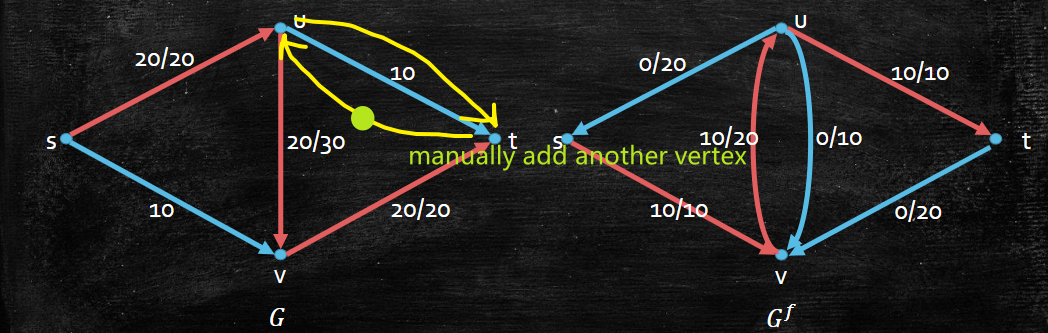
\includegraphics[width=0.8\linewidth]{Notes/fig/maxflow.png}
    \caption{Residual network}
    \label{fig:6-1}
\end{figure}

\begin{algorithm}
    \caption{Ford-Fulkerson algorithm}
    \KwIn{G=(V,E),s,t,c}
    \KwOut{f}
    initialize f s.t. $\forall e \in E$: f(e)=0; initialize $G^f=G$;\\
    \# Note that if both $(u,v)$ and $(v,u)$ exists, to avoid recursion , we add an extra vertex, as is shown in \ref{fig:6-1}.\\
    \While{there is an s-t path p on $G^f$}{
        find an edge $e \in p$ with minimum capacity b\\
        \ForEach{$e=(u,v)\in p$}{
            \If{$(u,v)\in E$}{
                update $f(e)=f(e)+b$\\
            }
            \If{$(v,u)\in E$}{
                update $f(e)=f(e)-b$\\
        }
        update $G^f$\\
        }
    }
    \Return{f}
\end{algorithm}
\subsubsection{Correctness of Algorithm}

Denote $c(S,T)=\sum_{e=(u,v),u\in P_s,v \in P_t} w(e)$, i.e. the number of edges from $P_s$ to $P_t$.
\textbf{Minimum cut problem} minimizes $c(S,T)$.\\
\begin{thm}
    \textbf{Max-Flow-min-cut Theorem:} 
    
    The value of the maximum flow is exactly the value of the minimum cut:
\[max_fv(f)=min_{S,T}c(S,T)\].
\end{thm}
\begin{figure}[htbp]
    \centering
    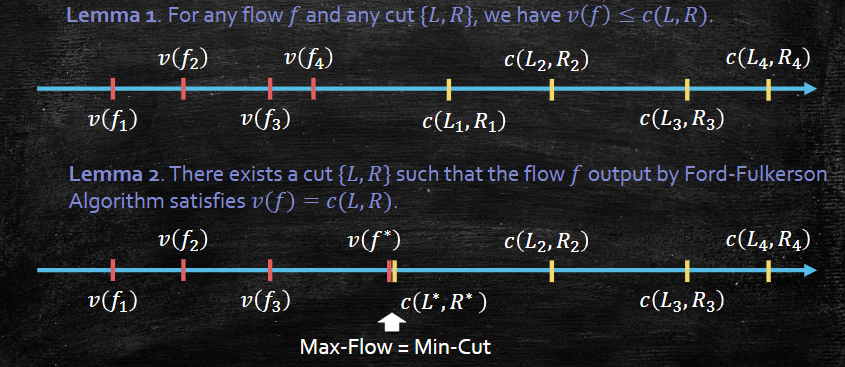
\includegraphics[width=0.7\linewidth]{Notes/fig/maxFlowProof.png}
    \caption{Proof of $f(S,T)=c(S,T)$}
    \label{fig:6-2}
\end{figure}
A visualization of proof is shown in \ref{fig:6-2}.
\begin{itemize}
    \item $max_fv(f)\leq min_{S,T}c(S,T)$\\
    To prove this, we will first prove $v(f)=f(S,T)-f(T,S)$. If this holds, then $v(f)=f(S,T)-f(T,S)\leq f(S,T)=\sum w(u,v)\leq \sum c(u,v)=c(S,T)$.

    $f^o(u)$ is flow leaving u, $f^i(u)$ is flow entering u.
    $\sum_{u\in S}(f^o(u)-f^i(u))=f^o(s)+\sum_{u\in L\setminus s}0=v(f)$

    $\sum_{u\in S\text{ or} T}(f^o(u)-f^i(u))=\sum_{u\in S,v\in T}f(u,v)-\sum_{u\in T,v\in S}f(u,v)$. which is intuitive. Consider three kinds of edge, if $u,v \in S$, $f^o(u)-f^i(v)=0$. If $u\in S, v\in T$, $f^o(u)-f^i(v)=f(u,v)$. If $u\in T, v\in S$, $f^o(u)-f^i(v)=-f(u,v)$. Putting them together we get the equation above.

    \item $\exists f \text{ produced by Ford-Fulkerson Algorithm satsifies:} v(f)= c(S,T)$
    Denote $S$ as vertice reachable from s in $G^f$.We'll prove that $f(S,T)=c(S,T)$, and $f(T,S)=0$. If $v(f)\leq c(S,T)$, at least an edge across the cut isn't full, so $(u,v)$ must occur in the residual network, u is reachable from v, which contradict with the definition of partition. Similarly ,we can prove $f(T,S)=0$

\end{itemize}
Therefore, we not only obtain a way to calculate maximum flow, but also minimum cut.
\subsubsection{Time Complexity}
Notice that min-cut is polynomial, but max-cut is NP-Hard.
If capacities are integers, then each while-loop at least increases $f$ by one, so it must terminate(after at most $f_max$ times).
If each $c(e)$ is an integer, then there exists a maximum flow $f$ such that $f(e)$ is an integer for each $e$.(exists a max flow version whose edges are all integer), as Ford-Fulkerson Algorithm can produce an integer-capacity flow.
With rational capacities, we can scale all numbers to integer. No need to consider irrational number, as they indeed will be presented as rational numbers in computer.
We do dfs once from $s$, points reachable from $s$ is less than $E$, $O(|V|+|E|)=O(|E|)$, with $f_max$ rounds, $O(|E|\cdot f_max)$(not polynomial).
Consider the following case \ref{fig:worseCase}, if at first you get $(u,v)$ iteratively, you will run 100000000 times, but if you get $s-u-t$ and then $s-v-t$, then you can end in 2 rounds.

For better choice of edge, we introduce Edmonds-Karp Algorithm.




\subsubsection{Edmonds-Karp Algorithm}
\begin{figure}[htbp]
    \centering
    \begin{minipage}{0.3\linewidth}
        \centering
        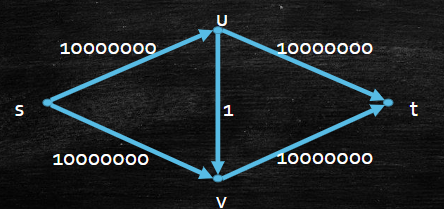
\includegraphics[width=1\linewidth]{Notes/fig/worseCase.png}
        \caption{Residual network}
        \label{fig:worseCase}
    \end{minipage}
    %\qquad
    \begin{minipage}{0.65\linewidth}
        \centering
        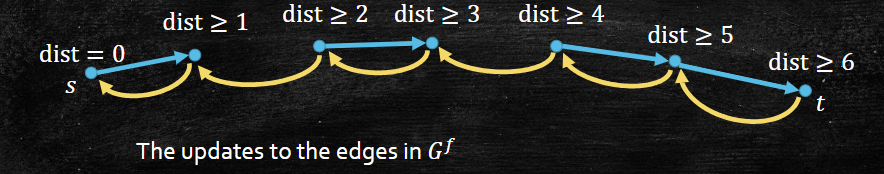
\includegraphics[width=1\linewidth]{Notes/fig/keyObservation.png}
        \caption{keyObservation}
        \label{fig:keyObservation}
    \end{minipage}
\end{figure}

In every update, at least an edge satuate in $G$ thus disapearing in $G^f$. Consider the new yellow edges in \ref{fig:keyObservation}, they won't decrease the distance between two vertice, so $dist(u)$ (=number of edges(steps) needed to reach u from s) is non-decreasing through out the algorithm. So the distance will only be increased $|V|+1$ times, and terminates after $O(|V|^2)$


Denote $f_i$ as the current-flow in $i^{th}$ iteration, $G^{f_i}$ is the residual graph after $i^{th}$ iteration of finding path. An edge $(u,v)$ is critical(satuated) if the amount of flow pushed along p is $c^{f_i}(u,v)$. We will proof that the number of times an edge becomes critical isn't big. Consider the things happening bewteen an edge becomes critical twice.
(u,v) in G, (v,u) in $G^f$, (v,u) in G,
But $dist(v)>dist(u)$ by BFS,
$dist^{i+j}(u)=dist^{i+j}(v)+1\geq dist^i(v)+1\geq dist^i(u)+2$

\begin{itemize}
\item distance of u to s increases by 2 between during the interval of an edge being "critical" twice.
\item Distance takes value from $\{0,1,\ldots,|V|,\infty\}$ and never decrease
\item When an edge is critical, the distance of its head increases by 1
\item each edge can only be critical for $O(|V|)$ times
\item At least one edge becomes critical in one iteration
\item total number of iterations is $O(|V||E|)$
\item each iteration takes $O(|E|)$ times
\item Overall time complexity takes $O(|V||E|^2)$
\end{itemize}


\begin{algorithm}
    \caption{Edmonds-Karp Algorithm}
    \KwIn{G=(V,E),s,t,c}
    \KwOut{f}
    initialize f s.t. $\forall e \in E$: f(e)=0; initialize $G^f=G$;\\
    \While{there is an s-t path p on $G^f$}{
        find a path $p$ by \textbf{BFS};\\
        find an edge $e \in p$ with minimum capacity b\\
        \ForEach{$e=(u,v)\in p$}{
            \If{$(u,v)\in E$}{
                update $f(e)=f(e)+b$\\
            }
            \If{$(v,u)\in E$}{
                update $f(e)=f(e)-b$\\
        }
        update $G^f$\\
        }
    }
    \Return{f}
\end{algorithm}

\subsection{Applications of Maximum Flow}
% introductions to algorithms
\subsubsection{Dinner Table Assignment}
Students from m different universities participate in a
conference. Each university i has $r_i$ students.
n tables, each table i can be shared by at most $c_i$ students
The problem has been transfered into whether max-flow has value $\sum_{i=1}^mr_i$
\begin{figure}
    \centering
    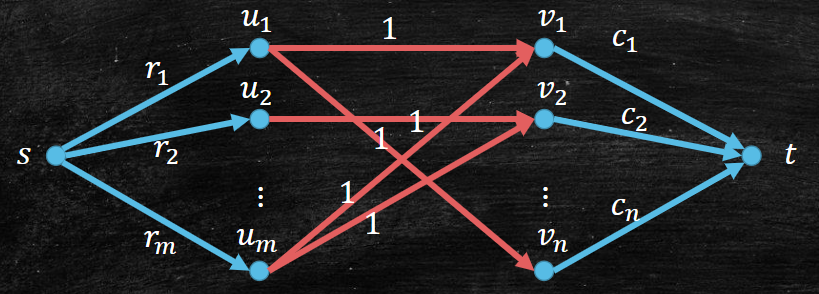
\includegraphics[width=0.5\linewidth]{Notes/fig/DTA.png}
    \caption{Dinner Tabel Assignment}
    \label{fig:DTA}
\end{figure}

\subsubsection{Tournament}
Four teams, whose wins are as follows: A=40, B=38, C=37, D=29, and the matches unfinished is marked on the graph.
\begin{figure}
    \centering
    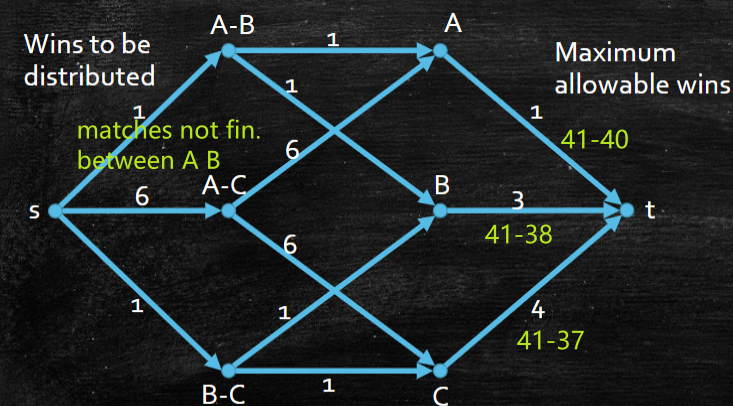
\includegraphics[width=0.5\linewidth]{Notes/fig/tournament.png}
    \caption{Tournament}
    \label{fig:tnm}
\end{figure}
If $f$ is 8, then theretically D can win.
\subsubsection{Maximum Bipartite Matching}
Example given in fig \ref{fig:MBM}. For vertice starting from $s$ or ending at $t$, capacity is 1. For other vertice, capacity is $\infty$. The maximum flow is equal to the maximum matching.
\begin{figure}
    \centering
    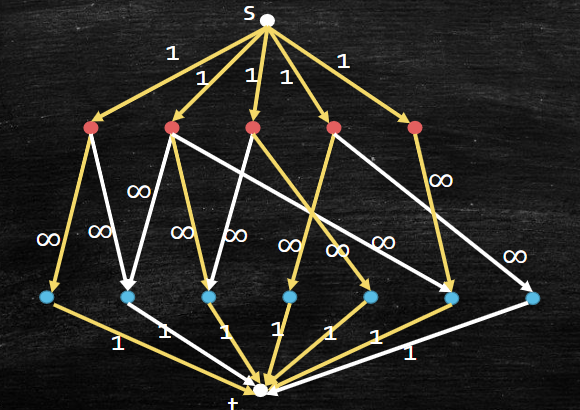
\includegraphics[width=0.5\linewidth]{Notes/fig/MaxMatching.png}
    \caption{change maximum matching into max flow}
    \label{fig:MBM}
\end{figure}
% dinic 

\subsection{Big Theorem for Maximum Flow on Bipartite Graph}

We will prove that the following four problems are equivalent for Bipartite Graph:
\begin{itemize}
    \item \textbf{Maximum Flow:} Max flow from $s$ to $t$ satisfying capacity and flow conservation constraints.
    \item \textbf{Minimum Cut:} $c(S,T)$ is the min sum of edge weight from $s$ to $t$ with minimum total capacity.
    \item \textbf{Maximum Independent Set:} $S\subseteq V$, no edge between any two vertices in $S$.
    \item \textbf{Minimum Vertex Cover:} $S\subseteq V$, $S$ contains at least one endpoint of each edge.
\end{itemize}
\[\text{The number of Maximum Flow= The number of minimum cut}\]
\[\text{The number of smallest vertex cover=$|V|$-The number of maximum independent set}\]
\begin{figure}[htbp]
    \centering
    \begin{minipage}{0.48\linewidth}
        \centering
        
\includegraphics[width=1\linewidth]{Notes/fig/relation_Flow.png}
        \caption{The proof pipeline of vertex cover, independent set, max flow and min cut on Bipartite Graph}
        \label{fig:MBG}
    \end{minipage}
    %\qquad
    \begin{minipage}{0.48\linewidth}
        \centering
        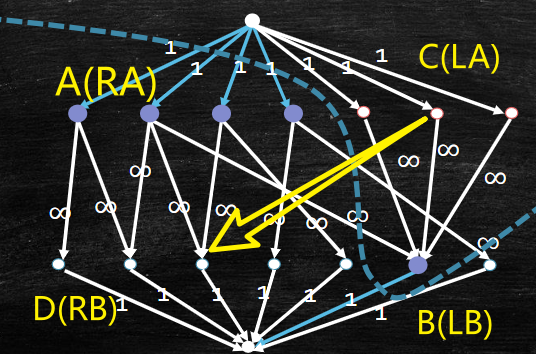
\includegraphics[width=0.8\linewidth]{Notes/fig/Network_Prove.png}
        \caption{num of white edges ending at t are the max flow; blue edges are the min cut; purple vertice are the minimum cover; white vertice are the maximum independent set}
        \label{fig:Network_Prove}
    \end{minipage}
\end{figure}
The main pipeline is shown in fig \ref{fig:MBG}. We will prove the following four statements:
\begin{itemize}
    \item Maximum Independent Set $\Leftrightarrow$ Minimum Vertex Cover\\
    $S$ is an Independent set iff $V\setminus S$ is a vertex cover. Intuitively, when finding an independent set, edges are $\bullet -\circ$ or $\circ - \circ$, while finding a vertex cover, edges are $\circ - \bullet $ or $\bullet - \bullet$. For every edge in an independent set $S$, at least one of its endpoint must be in $V\setminus S$, else an edge exists between vertice in $S$.  Consider $V \setminus S$, it forms a vertex cover, since all vertice connected to $S$ are in $V\setminus S$.
    Therefore, maximum independent set is equal to $|V|$-minimum vertex cover.

    \item Min Vertex Cover $\Leftrightarrow$ Min-Cut\\
    By the operation of max flow, $c(\{s\}\cup C\cup B, \{t\}\cup D\cup A)=c(s,A)+c(B,t)$, since $c(B,D)=c(C,A)=0$ by the definition of Bipartite Graph, $c(B,A)=0$ by the direction of edges, $c(C,D)=0$, else min-cut goes to infinity. $c=|A|+|B|$, since $w(s,a\in A)=1$. $A\cup B$ forms a vertex cover in the original undirected Bipartite Graph. If there exists $e=(u,v)$, $u,v \notin A \cup B$, $u\in C, v \in D$, contradiction!
    Suppose $A\cup B$ is a vertex cover, then there is no edge from $C$ to $D$, else an edge isn't covered, contradiction! $\{s\}\cup C\cup B, \{t\}\cup D\cup A$ is a cut whose size is $|A|+|B|$ by similar approach. Therefore, min-cut is equal to min vertex cover.
    \item Min-Cut $\Leftrightarrow$ Max-Flow
    
    Proven by Max-Flow-Min-Cut Theorem. Notice that when algorithm terminates, the points reachable from s but not t forms $F$, where minimum cut is $c(F, V\setminus F)$. The vertice set of cut-edges forms a vertice cover, as its complement is an independent set. 
    \item Max Flow $\Leftrightarrow$ Maximum Matching
    constructed in fig\ref{fig:MBM}.
    All matching problems can be solved in polynomial time
\end{itemize}

For a general graph, although finding a min vertex cover is np-hard, we can still find a 2-approximation based on maximal matching:
\begin{itemize}
    \item The set of endpoints for all edges in a maximal matching is
    a vertex cover.\\
    Since for any edge $e=(u,v)$, one or both of u,v must be an endpoint of an edge in $M$. Otherwise, $M \cup \{e\}$ is still a matching, and  $M$ is not maximal
    \item For any maximal matching $M$, the size of any vertex cover is at least $|M|$.\\
    Since at least a vertex in a matching will be chosen.(Consider the extreme case )
    \item Since $|S(G)|=2|M|$, $OPT(G)\geq |M|$, we successfully find a 2-approximation
\end{itemize}